\section{Beading strategies}
Now that we have described a framework for deciding and applying on bead counts and their widths locally, we can introduce several beading strategies which determine the bead count and their widths in different ways.
We can emulate a variety of toolpath generation methods from related literature by meticulously defining new beading strategies.
We also introduce new beading strategies which produce toolpaths with less extremal widths then techniques from existing literature.

A beading strategy was defined as a set of some particular variables and functions (\cref{beading_strategy_definition}).
Our beading strategies are based on a preferred width $w_\text{pref} = \SI{0.4}{\milli\meter}$, which is equal to the size of the hole in the printing nozzle.
Most of the beading strategies we introduce share a common ground:
\begin{align*}
d_\text{max}^\text{transition} &= \SI{1}{\milli\meter} \\
d^\text{discretization} &= \SI{0.2}{\milli\meter} \\
t_\text{beading} &= w_\text{pref} \\
d_\text{max}^\text{intersection} &= \SI{75}{\percent} \\
%
%We use a transition anchor position of
%$$t_-(n) =  t(n) \frac{ b^{-1}(n) - p(n) }{p(n+1) - p(n) }$$
%$$t_-(n) =  t(n) \frac{ b^{-1}(n) - 0.4n }{0.4(n+1) - 0.4n }$$
%$$t_-(n) =  t(n) \frac{ b^{-1}(n) - 0.4n }{0.4}$$
t_0(n) &=  t(n) \left( b^{-1}(n) / w_\text{pref}  - n \right) \\
t(n) &= w_\text{pref} \\
\alpha_\text{max} &= \SI{135}{\degree} \\
L(n,d)_i &= 
\begin{cases}
-\frac12 W(n,d)_i + \sum_{j=0}^i W(n,d)_j & \text{ if } i < \frac12 (n -1) \\
d/2 & \text{ if } i =  \frac12 (n -1) \\
d - W(n,d)_{n-1-i} & \text{ otherwise }\\
\end{cases}
\end{align*}

The transition anchor position $t_0$ ensures that the transitions never overlap with the locations $v$ where $2 R(v) = n w_\text{pref}$ for $n \in \mathbb{N}$.
The transition length $t$ ensures that the center beads don't overlap with the innermost transitioning beads, while keeping the amount of underfill low and keeping the toolpath smooth.
The limit bisector angle $\alpha_\text{max}$ ensures that we don't employ transitioning in shallow wedge regions, which would result in a lot of short odd single bead polylines, which would break up the semi-continuous nature of polygonal extrusion paths.
The toolpath locations $L$ ensure that beads are extruded from the center of where they end up, that the beads don't overlap and that the symmetry restrictions are met.


\paragraph{Naive Beading Strategy}
We can define a beading strategy which emulates the naive method by disabling the marking of edges, so that we never employ transitioning.
\begin{align*}
\alpha_\text{max} &= \SI{180}{\degree} \\
b^-(d) &= 2 \left\lfloor \frac{d}{ 2w_\text{pref}} + \frac12 \right\rfloor \\
W(n,d)_i &= w_\text{pref} \text{ for all } i 
%\\
%L(n,d)_i &= w_\text{pref} \left(i + \frac12 \right) \text{ for all } i < \frac12 n
\end{align*}



\paragraph{Outer bead}
We can emulate the method by \citeauthor{Moesen2011} by carefully choosing how the beading strategy functions deal with the outermost bead.
Also we turn off the reduction of line segments near 3-way intersections, so that the polygonal toolpaths emulate the remaining area to be filled by another path planning technique similar to their technique.

\begin{align*}
d_\text{max}^\text{intersection} &= \SI{0}{\percent} \\
t(n) &= 0 \\
b(d) &=
\begin{cases}
1 & \text{ if } d < w_\text{pref} \\
2 & \text{ otherwise } \\
\end{cases}
 \\
W(n,d)_i &= 
\begin{cases}
d & \text{ if } n = 1 \\
w_\text{pref} & \text{ otherwise } \\
\end{cases}
%\\
%L(n,d)_i &= 
%\begin{cases}
%d / 2 & \text{ if } n = 1 \\
%w_\text{pref} / 2 & \text{ otherwise } \\
%\end{cases}
\end{align*}


\paragraph{Constant bead count}
We can emulate the method by \citeauthor{Ding2016a}, by dividing the feature diameter over the widths of a constant number of beads.
Additionally in order to emulate their definition of branches we mark all segments and in a separate algorithm we unmark the outer bones connected to the outline shape.
Note that this deviation from the proposed framework violates the robustness against small perturbations in the outline polygon, since the topology of the skeletal graph is not stable against those.

\begin{align*}
\alpha_\text{max} &= \SI{0}{\degree} \\
b(d) &= C \\
W(n,d)_i &= d / n \text{ for all } i 
%\\
%L(n,d)_i &= d / n \left(i + \frac12 \right) \text{ for all } i < \frac12 n
\end{align*}



\paragraph{Centered}
We can emulate the method by \citeauthor{Jin2017JMS}, by transcribing how they deviate from the naive tool paths.
We therefore base the beading strategy on the bead count $b^(d)$ defined by the naive beading strategy.
\citeauthor{Jin2017JMS} replace two beads from the naive toolpaths by a single one when the radius between the center and either of those beads falls short of $r_\text{min} = 0.8 w_\text{pref}$.
Conversely, they place an extra bead when the radius between the center and either of the innermost beads exceeds $r_\text{max} = 1.25 w_\text{pref}$.\cite{Jin2017JMS}
We emulate the rounded polygonal path rerouting they define by supplying a transition length which results in a discretized version of the rounded polygon segment.

\begin{align*}
t(n) &= \frac12 w_\text{pref} \\
b^-(d) &= 2 \left\lfloor \frac{d}{ 2w_\text{pref}} + \frac12 \right\rfloor \\
b(d) &= b^-(d) +
\begin{cases}
-1 & \text{ if } b^-(d) w_\text{pref} - d > w_\text{pref} - r_\text{max} \\
1  & \text{ if }  b^-(d) w_\text{pref} - d < w_\text{pref} - r_\text{min} \\
0 & \text{ otherwise}
\end{cases}
\\
W(n,d)_i &= 
\begin{cases}
d - (n-1) w_\text{pref} &\text{ if } i = \frac12 (n-1) \\
w_\text{pref} &\text{ otherwise }
\end{cases}
%\\
%L(n,d)_i &= 
%\begin{cases}
%d / 2 & \text{ if } i = \frac12 (n-1) \\
%w_\text{pref} \left(i + \frac12 \right) & \text{ otherwise }
%\end{cases}
\end{align*}





\paragraph{Evenly distributed}
By taking the advantages of the above two strategies we can define a beading strategy which constitutes a novel toolpathing technique.
We can evenly divide the local feature diameter over the widths of all beads, but choose a local bead count better matching the local feature size.
We determine the local bead count by dividing the diameter by the prefered bead width and rounding to the nearest integer.
This reduces the demands on the system and deviation from mechanical properties caused by beads with extreme deviations from the preferred width.



\begin{align*}
b(d) &= \left\lfloor \frac{d}{ w_\text{pref}} + \frac12 \right\rfloor \\
W(n,d)_i &= d / n \text{ for all } i 
%\\
%L(n,d)_i &= d / n (i + \frac12) \text{ for all } i < \frac12 n
\end{align*}




\paragraph{General distributed strategy}
The evenly distributed strategy can be conceptualized as calculating the total discrepancy $E$ between the actual feature diameter $d$ and the total preferred width $n w_\text{pref}$, dividing the total discrepancy by the number of beads and setting the width of each bead to 
$w_\text{pref} + E / n$.
However, depending on the application we might want a different distribution of widths.
We therefore supply a beading strategy which supports an arbitrary distribution of the discrepancy.
The distribution is determined by some weighing function $M(n.d)$, which defines the portion of the discrepancy to distribute to each bead.


\begin{align*}
b(d) &= \left\lfloor \frac{d}{ w_\text{pref}} + \frac12 \right\rfloor \\
E(n,d) &= d - n w_\text{pref} \\
W(n,d)_i &= w_\text{pref} + E(n,d) \frac{M(n,d)_i}{\sum_{j=0}^{n-1} M(n,d)_j} \text{ for all } i 
%\\
%L(n,d)_i &= d / n (i + \frac12) \text{ for all } i < \frac12 n
\end{align*}


\paragraph{Inward distributed}
For example, we can choose 
$$M(n,d)_i = \max(0, 1 - \frac{1}{N^2} (i - (n-1)/2)^2 )$$
to distribute the discrepancy over the innermost $2N$ beads, and distribute most of it to the inner beads.
That way we limit the region of impact of the distributed strategy to a central region and have the nominal bead width $w_\text{pref}$ in regions farther away.
This limits the impact of transitioning regions so that transitions keep the toolpaths smooth farther away from the central regions. % and it forces most of the beads to have exactly the prefered width.
Moreover, the bead widths equal the nominal bead width for large regions meaning that mechanial properties derived for prints using hte naive strategy will still hold approximately.




\paragraph{Widening}
Complementary to any of these strategies we can enforce a minimum feature size at no extra cost in our framework.
Regions where the model is narrower than the nozzle size can be printed with a bead width larger than the model thickness.
We can simply override
\begin{align*}
W'(n,d)_1 &=
\begin{cases}
\max \left( w_\text{nozzle}  ,  W(n,d)_1 \right) & \text{ if } n = 1 \\
W(n,d)_1 & \text{ otherwise}
\end{cases}
\end{align*}




















\section{Validation}
In order to test our framework we have assembled a data set of various types of 3D model, ranging over various applications and various types of geometry.
The dataset is described in detail in the accompanying data in \cref{dataset}.
We sliced all models in the data set and selected 300 random slices from the total set of slices.

\todo{describe dataset of 3d models and random slices... X number of 3d files. varying in size, topology, features (size). random selection of slices. 300 slices total.  5 toolpath strategies were applied for each layer.}

\begin{figure*}
\centering
\setlength{\figwidth}{0.19\textwidth}
\setlength{\figheight}{0.283\textwidth}
\begin{subfigure}{\figwidth}\centering
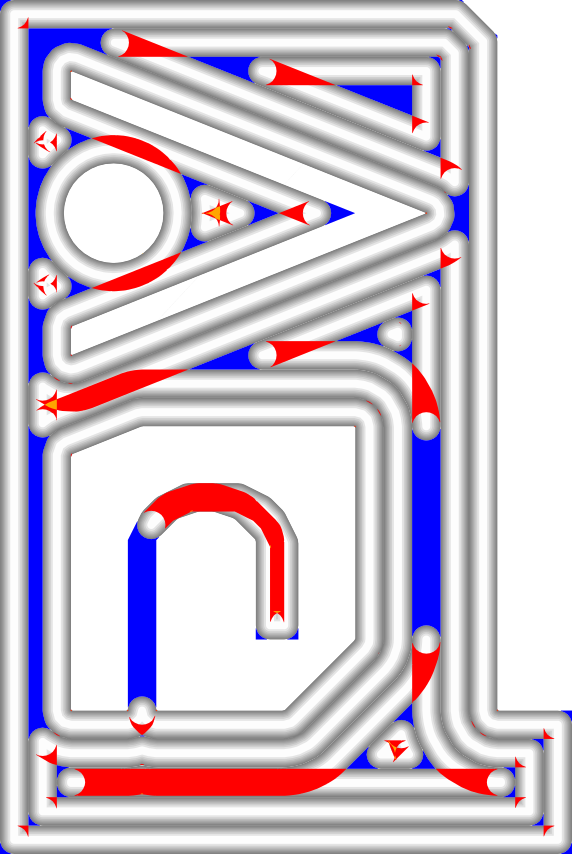
\includegraphics[height=\figheight]{sources/validation/gMAT_example/TEST_naive_accuracy.png}
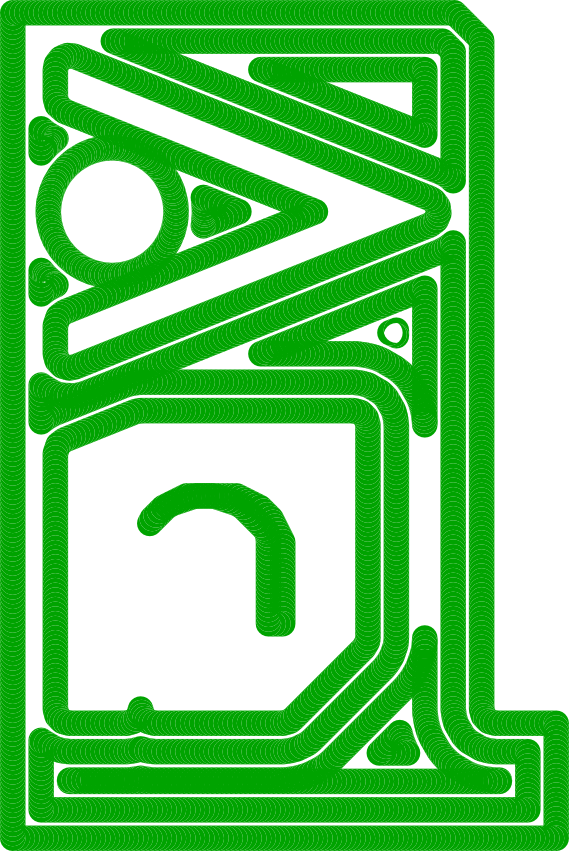
\includegraphics[height=\figheight]{sources/validation/gMAT_example/TEST_naive_widths.png}
\caption{Naive}\label{TEST_naive_accuracy}
\end{subfigure}
%\begin{subfigure}{\figwidth}\centering
%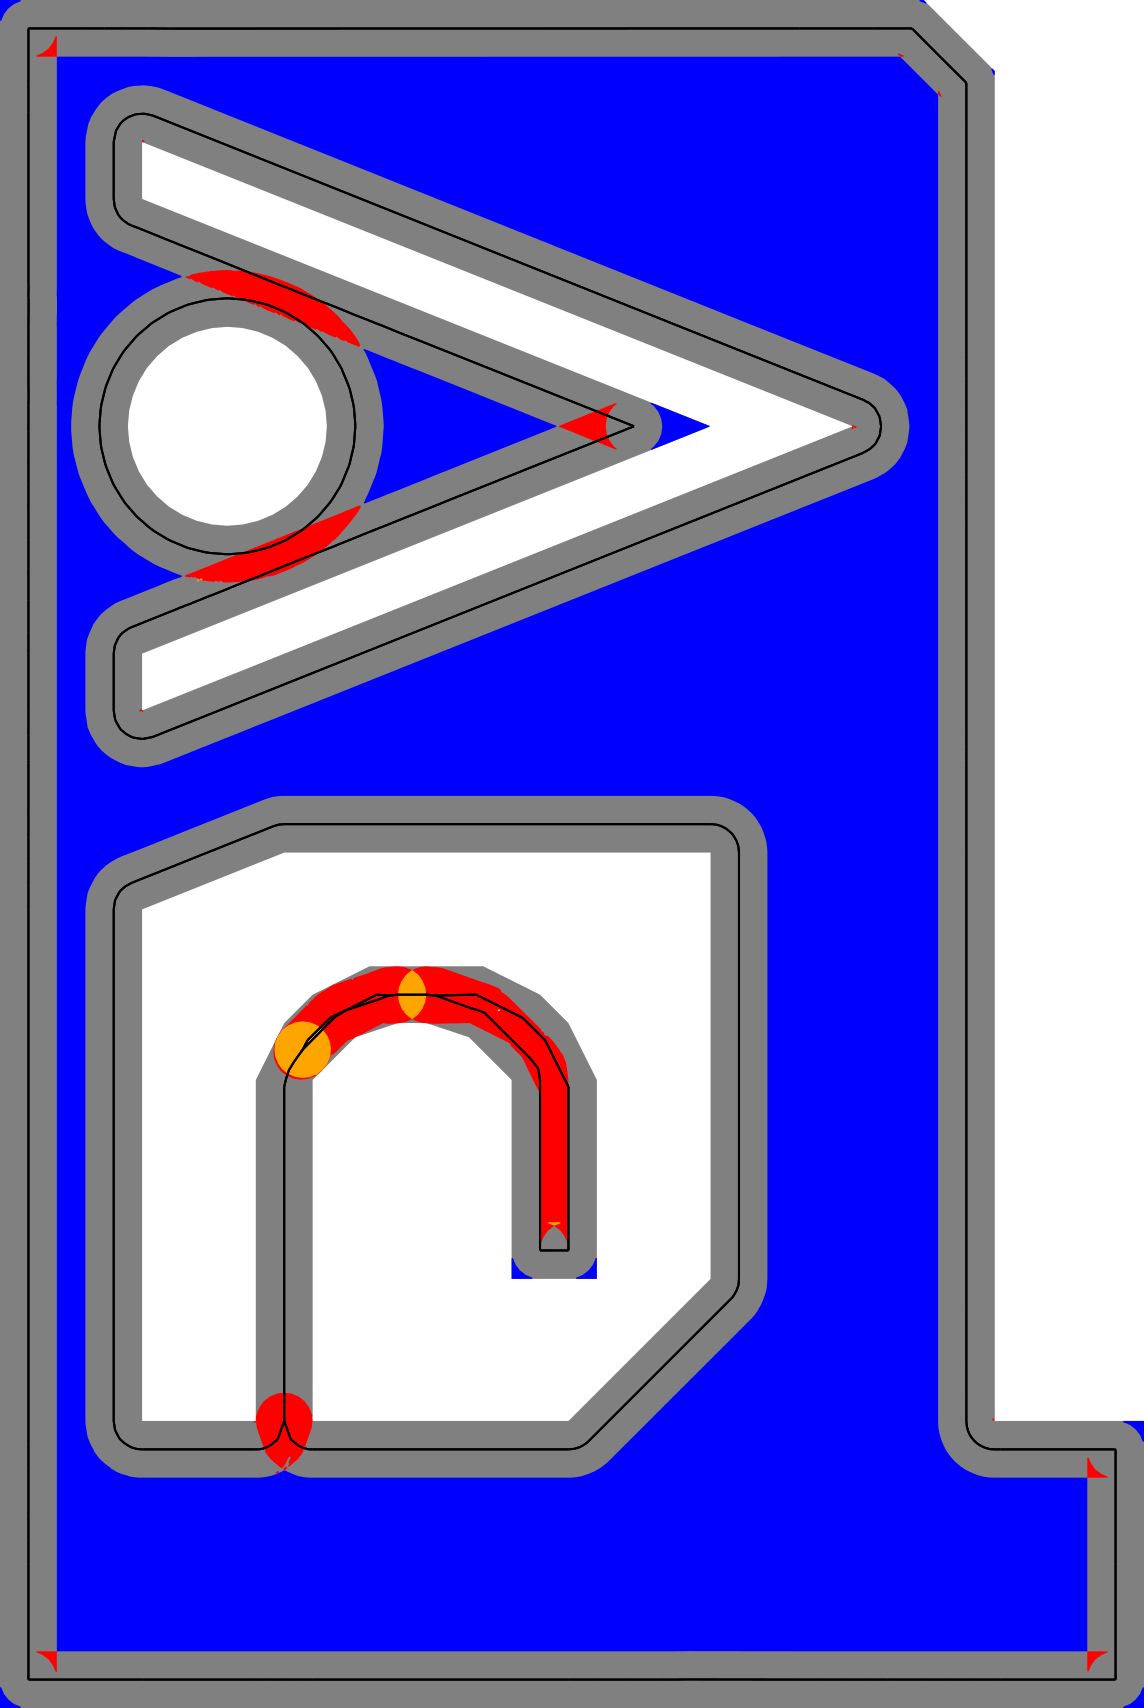
\includegraphics[height=\figheight]{sources/validation/gMAT_example/TEST_SingleBead_accuracy.png}
%
\includegraphics[height=\figheight]{sources/validation/gMAT_example/TEST_SingleBead_widths.png}
%\caption{Single}\label{TEST_SingleBead_accuracy}
%\end{subfigure}
\begin{subfigure}{\figwidth}\centering
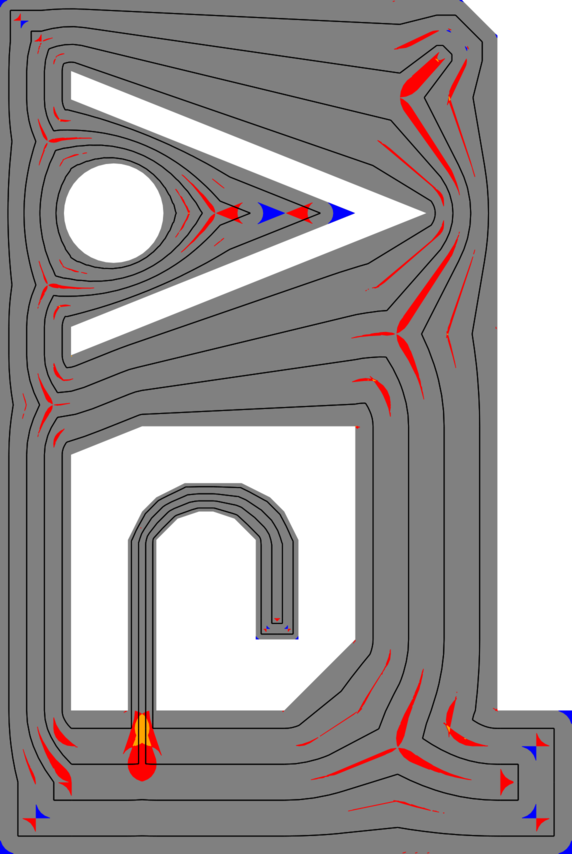
\includegraphics[height=\figheight]{sources/validation/gMAT_example/TEST_Constant_accuracy.png}
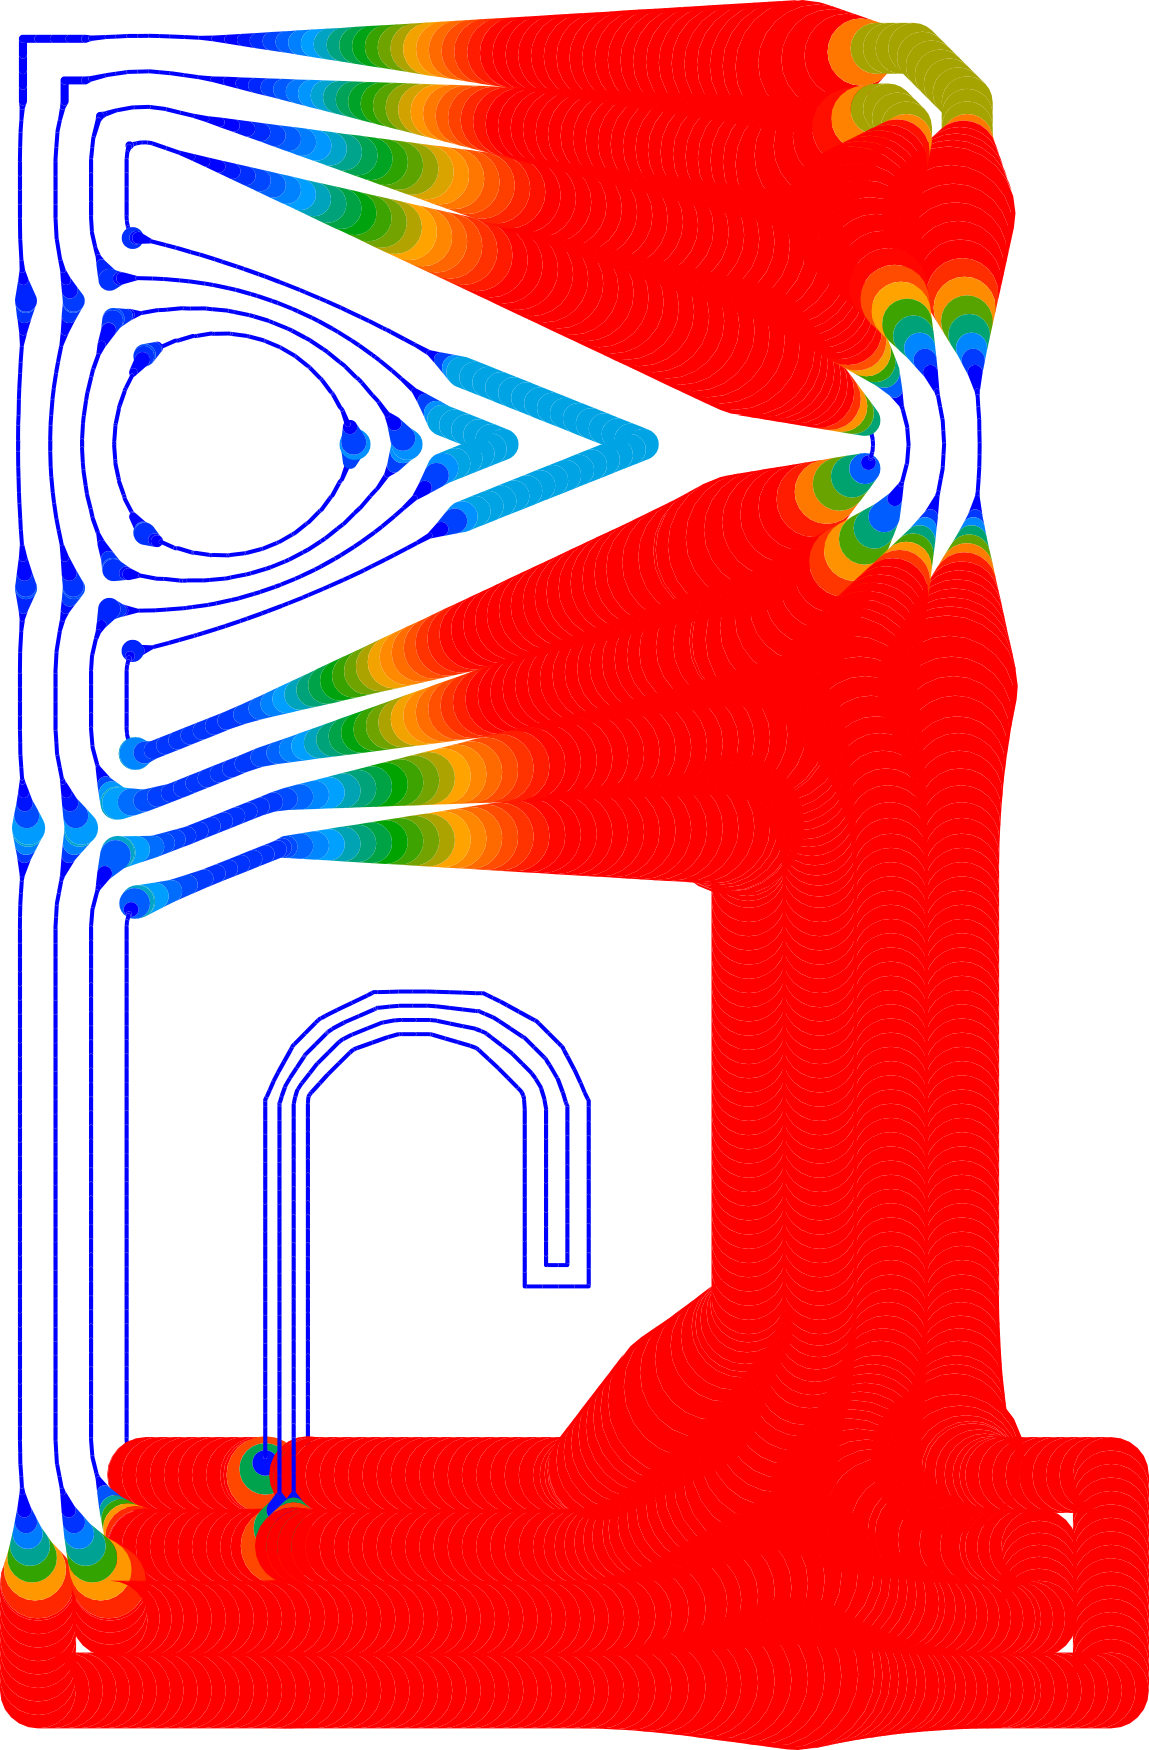
\includegraphics[height=\figheight]{sources/validation/gMAT_example/TEST_Constant_widths.png}
\caption{Constant}\label{TEST_Constant_accuracy}
\end{subfigure}
\begin{subfigure}{\figwidth}\centering
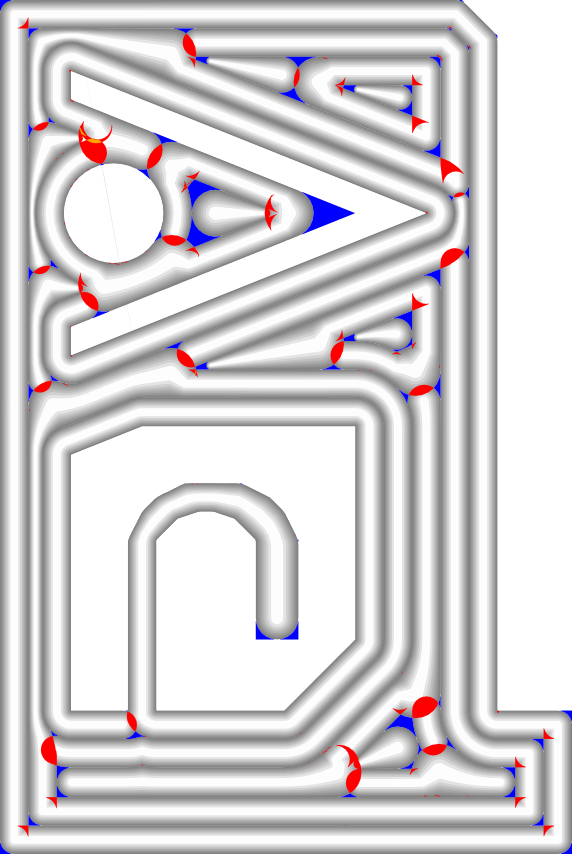
\includegraphics[height=\figheight]{sources/validation/gMAT_example/TEST_Center_accuracy.png}
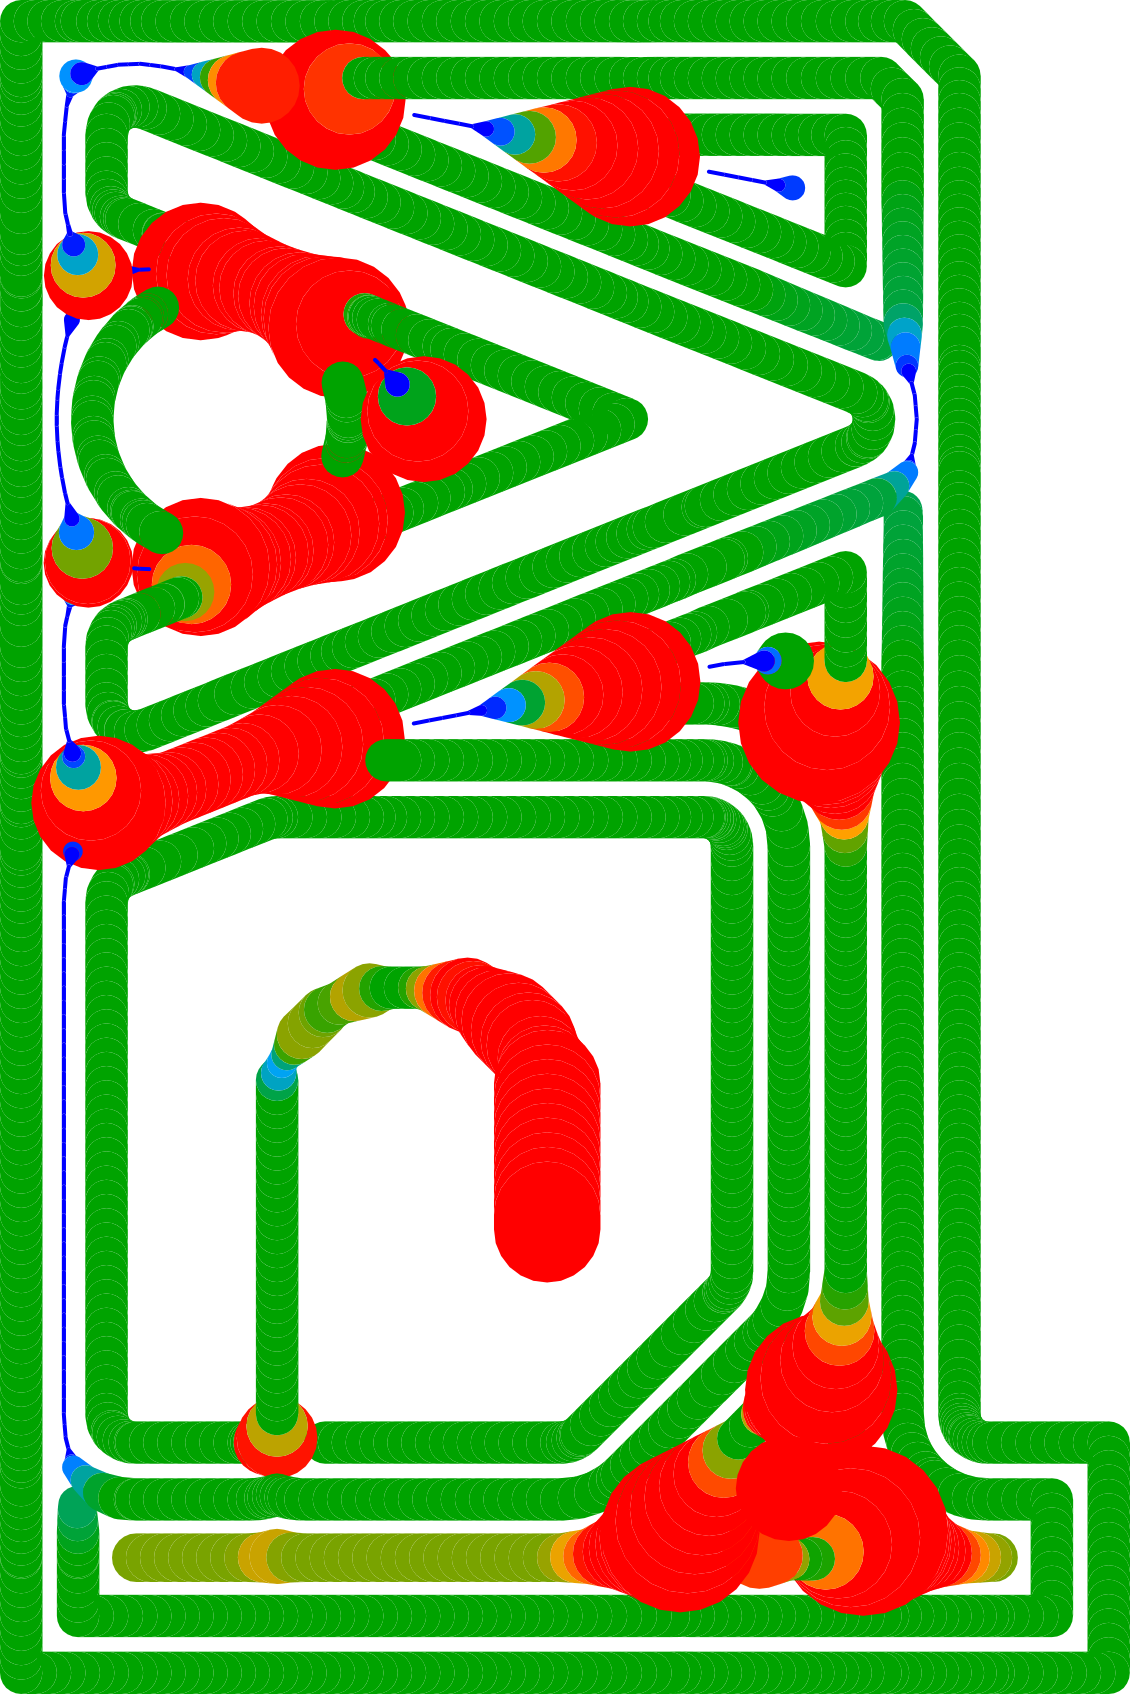
\includegraphics[height=\figheight]{sources/validation/gMAT_example/TEST_Center_widths.png}
\caption{Center}\label{TEST_Center_accuracy}
\end{subfigure}
\begin{subfigure}{\figwidth}\centering
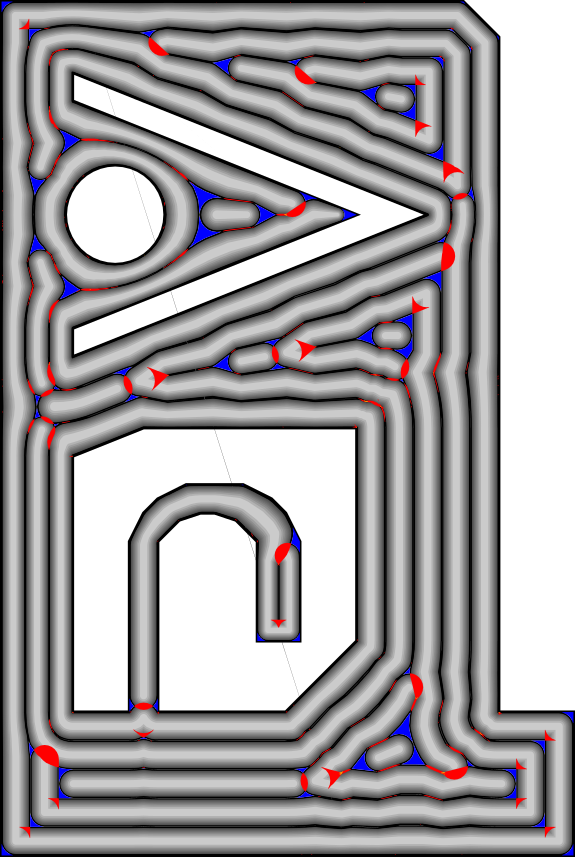
\includegraphics[height=\figheight]{sources/validation/gMAT_example/TEST_Distributed_accuracy.png}
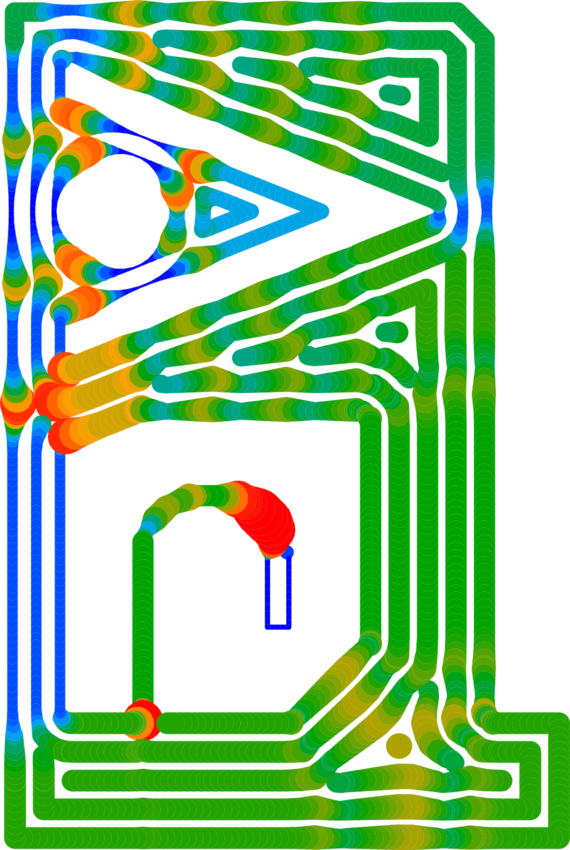
\includegraphics[height=\figheight]{sources/validation/gMAT_example/TEST_Distributed_widths.png}
\caption{Distributed}\label{TEST_Distributed_accuracy}
\end{subfigure}
\begin{subfigure}{\figwidth}\centering
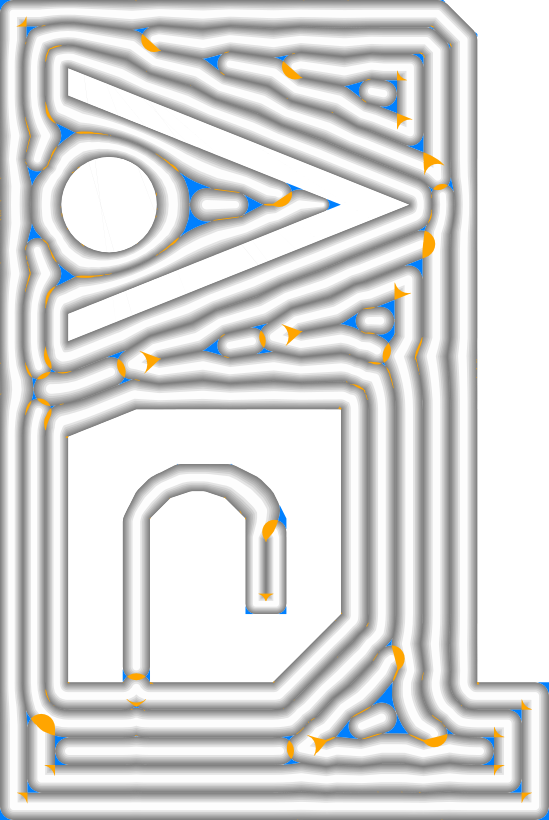
\includegraphics[width=\columnwidth]{sources/validation/gMAT_example/TEST_InwardDistributed_accuracy.png}
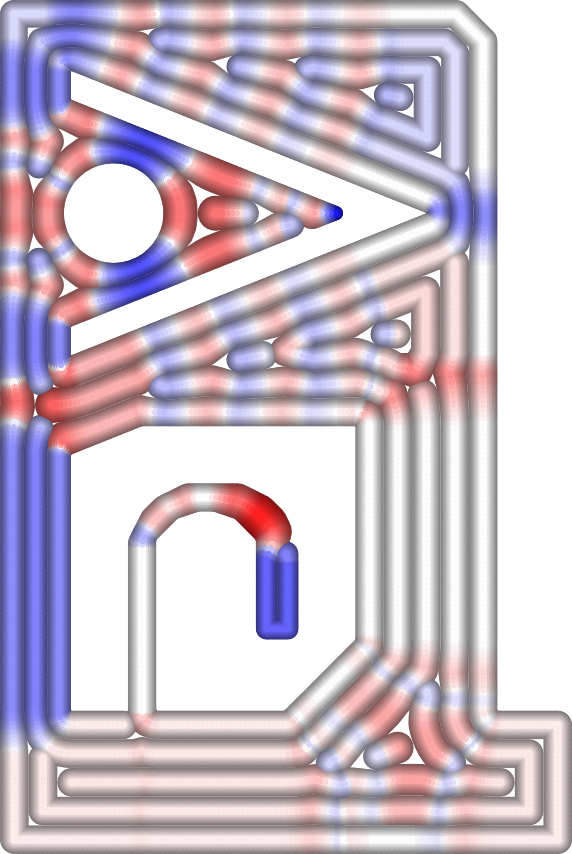
\includegraphics[width=\columnwidth]{sources/validation/gMAT_example/TEST_InwardDistributed_widths.png}
\caption{Inward}\label{TEST_InwardDistributed_accuracy}
\end{subfigure}
\begin{subfigure}{.04\columnwidth}\centering
\vspace{4cm}
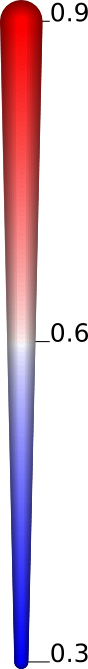
\includegraphics[height=\figheight]{sources/validation/gMAT_example/widths_legend.png}
\end{subfigure}
\caption{
Visualizing the overfills and underfills and the exaggerated widths for various beading strategies.
Grey areas are covered by extruded material,
blue areas in the top images signify underfill regions,
red areas overfill,
orange areas triply extruded areas (double overfill).
The bottom visualizes the bead widths at each location by exaggerating their widths.
Cold colors are narrower than the nozzle size and warm colors are wider than the nozzle size.
}
\label{visualized_accuracy}
\end{figure*}








\subsection{Computational analysis}
Experiments were performed on an Intel Core i7-7500U CPU @ \SI{2.70}{\giga\hertz} using a single core and \SI{16.3}{\giga\byte} memory.
The naive method was implemented using the state-of-the-art polygon offset library Clipper. \cite{johnson2014clipper}
The computation time of each slice from the dataset was recorded for the "Inward distributed" and "Naive" strategy. 
\cref{computime} shows these computation times of each layer plotted against the vertex count of the layer.

\paragraph{Accuracy}
In order to estimate the overfill and underfill, we need to accurately calculate the area covered by a single extrusion path.
If we would simply use an isosceles trapezoidal area with base lengths equal to the widths of the two end points of the segment, we would get strange artifacts at corners in the toolpath.
We therefore use a semi-circle with a diameter equal to the starting width in the one end of each segment, and exclude it at the other end, because it will be included in the next segment.
For polyline extrusion paths which are not closed, we also include the semi-circle corresponding to the extrusion width of the end-position.
In order to print such extrusion paths accurately, we can modulate the amount of material flow per millimeter based on this visualization model.
See \cref{segment_visualization}.

\begin{figure}
\centering
\setlength{\figwidth}{.25\columnwidth}
\begin{subfigure}{\figwidth}\centering
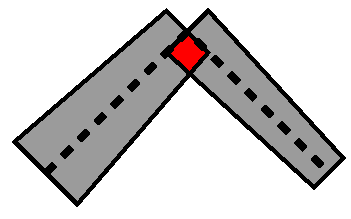
\includegraphics[width=\columnwidth]{sources/validation/visualization_principle_blocky.pdf}
\caption{Blocky}
\end{subfigure}
\begin{subfigure}{\figwidth}\centering
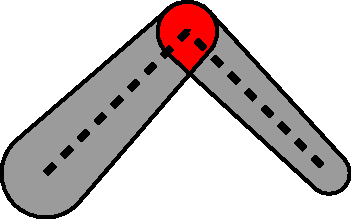
\includegraphics[width=\columnwidth]{sources/validation/visualization_principle_rounded.pdf}
\caption{Rounded}
\end{subfigure}
\begin{subfigure}{\figwidth}\centering
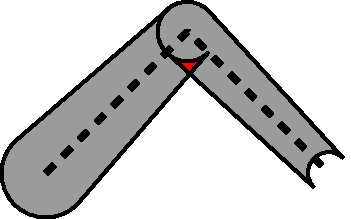
\includegraphics[width=\columnwidth]{sources/validation/visualization_principle_rounded_excluded.pdf}
\caption{Excluded}
\end{subfigure}
\caption{
Extruded area of two extrusion toolpath segments.
Red areas signify doubly extruded areas.
}
\label{segment_visualization}
\end{figure}

We can then estimate the amount of underfill by unioning the rounded visualization of all extrusion segments and then taking the difference from the original outline shape.
In order to deal with rounding errors, we perform a morphological close of \SI{5}{\micro\meter} before calculating the total area of the underfill regions.

The overfill regions are calculated by adding the polygonal areas of each extrusion segment to a list.
We then add the original outline shape in reverse and perform a clipper operation which only keeps areas of positive winding order.
Because the reverse outline shape reduces the winding order of all extruded segments by one, we are left with the overfill areas.
In order to estimate the areas which are triply covered by extrusion segments, we repeat the process of adding the outline in reverse and performing the clipper operation.
These triple extrusion areas count double toward the total amount of overfill.
The resulting overfill and underfill areas are visualized for the different toolpath strategies in the top of \cref{visualized_accuracy}.

We calculated the total overfill and underfill areas of the different toolpath strategies applied on the dataset. 
The overfill and underfill area as a percentage of the total area of the slices from the dataset are illustrated in \cref{over_underfill}.  
The "Inward distributed" strategy has a calculated overfill of 0.24\% and an underfill of 0.17\%.
This is lower compared to the "Naive" strategy, which results in 1.2\% overfill and 1.7\% underfill when applied to on dataset.

\begin{figure}
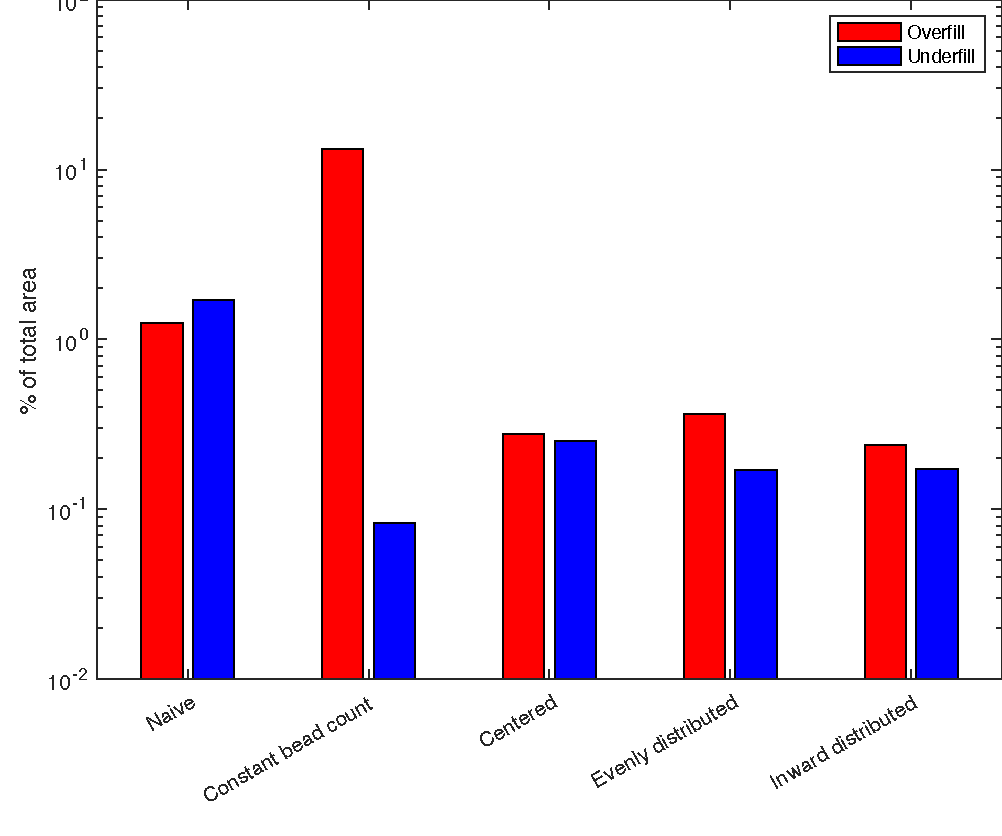
\includegraphics[width=\columnwidth]{sources/validation/overunderfill.pdf}
\caption{total over and underfill for entire dataset}
\label{over_underfill}
\end{figure}

\begin{figure}
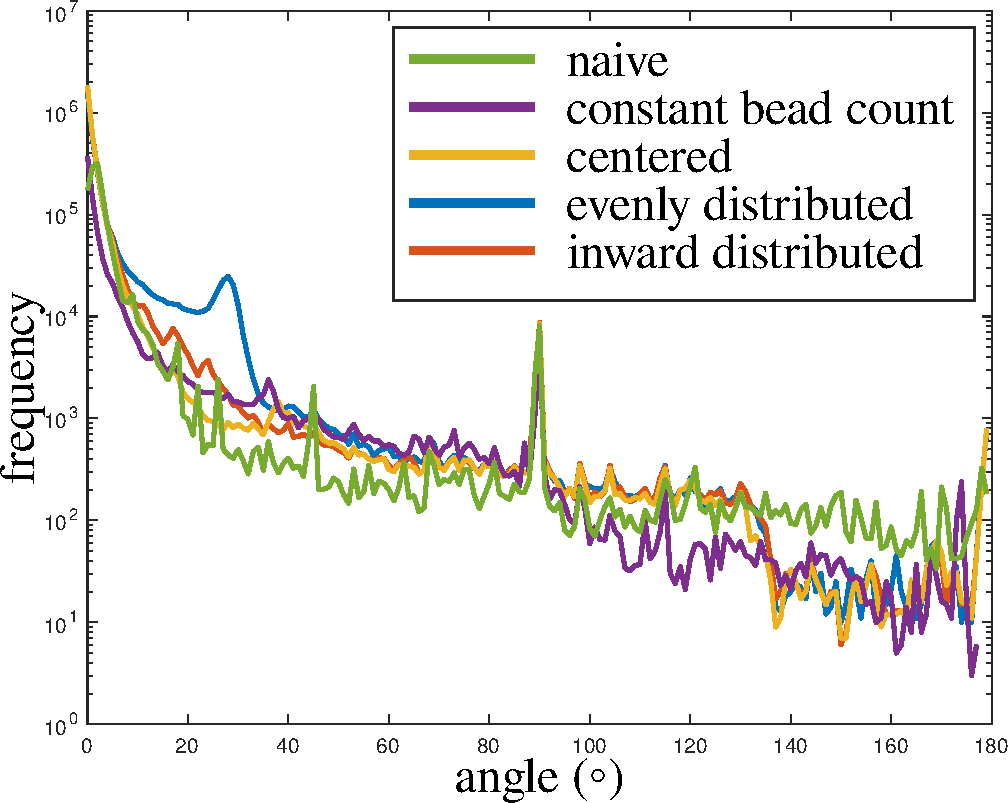
\includegraphics[width=\columnwidth]{sources/validation/smoothness.pdf}
\caption{occurrence of angles between consecutive segments}
\label{smoothness}
\end{figure}

\begin{figure}
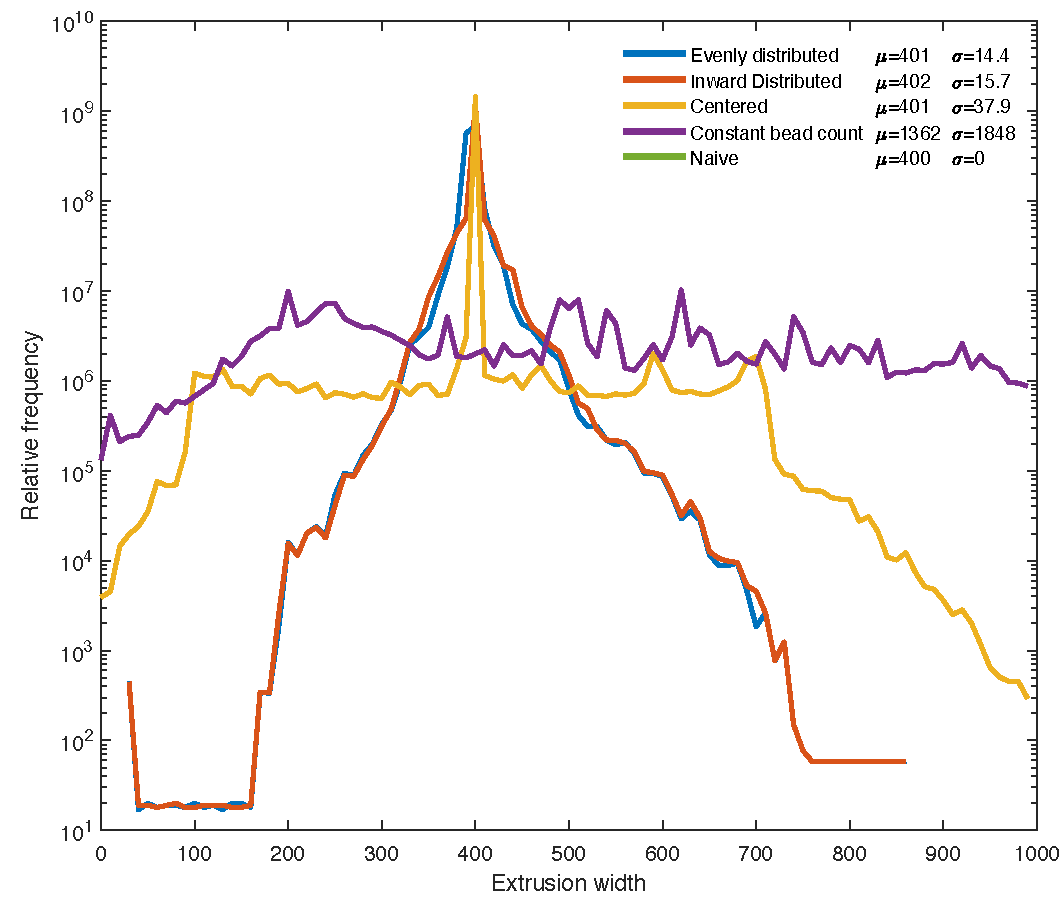
\includegraphics[width=\columnwidth]{sources/validation/widthHistogram.pdf}
\caption{Distribution of extrusion width, sampled at  \SI{200}{\micro\meter}, visualized data is binned at intervals of  \SI{10}{\micro\meter}}
\label{widthHistogram}
\end{figure}

\begin{figure}
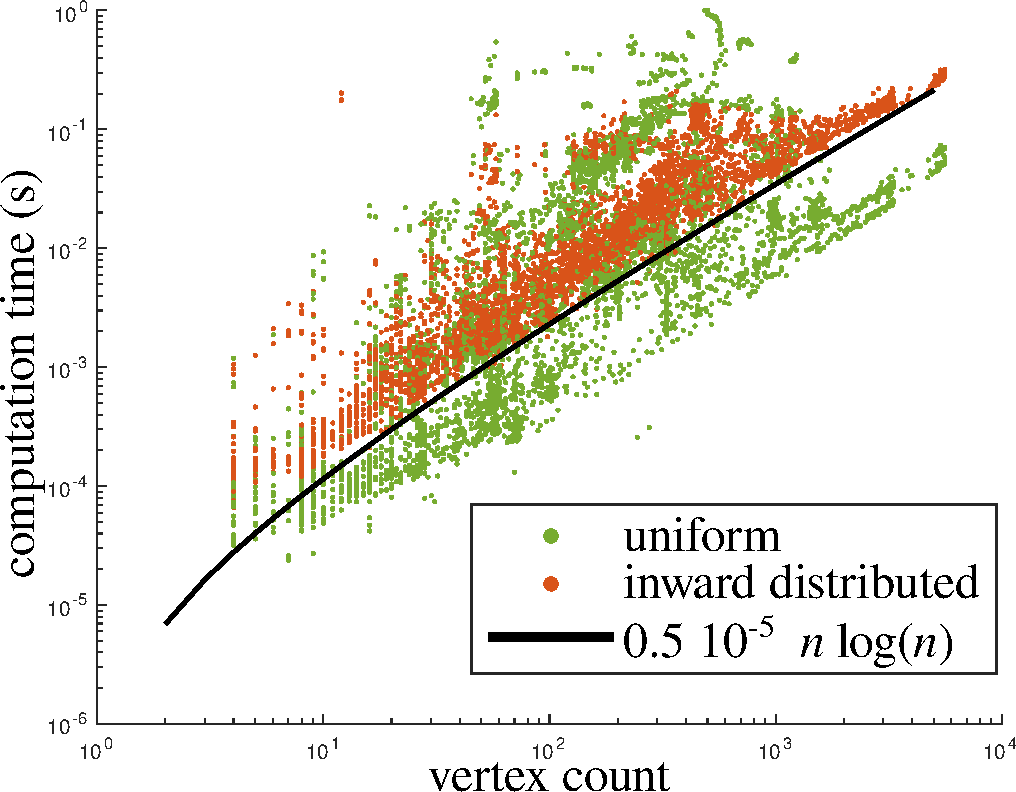
\includegraphics[width=\columnwidth]{sources/validation/computime2.pdf}
\caption{Computation time per slice}
\label{computime}
\end{figure}


\paragraph{Uniformity}
Depending on the printer hardware configuration, some bead widths might be difficult or impossible to manufacture.
A bead width far below the nozzle size can result in fluttered extrusion, while a bead width far above the nozzle size can require pressures above the specifications of the machine. 
Also, large bead widths can cause the extruded material to upwards instead of filling the required width.
\todo{Include picture of flutter?}
Moreover, bead widths deviating from the nominal bead width by a large amount may impact the mechanical properties of the print.
We visualize the bead widths resulting from the different strategies in an exaggerated manner in the bottom of \cref{visualized_accuracy}.

To evaluate the width uniformity, we sampled the extrusion widths of all generated toolpaths 
at intervals of \SI{200}{\micro\meter} along the toolpath.
From these sampled values, we calculated the mean bead width, and standard deviation.
\cref{widthHistogram} shows the distribution of extrusion width for each strategy.
The results show that the mean width of our strategies "Inwards distributed" and "Evenly distributed" is close to nominal nozzle size of \SI{400}{\micro\meter}, while their standard deviation is lower than for strategies "Centered" and "Constant bead count". 
These values indicate that, while causing less overfill and underfill, our strategy deviates less and less often from the nominal nozzle size.

\paragraph{Smoothness of toolpaths}
In order to maintain a high printing speed, it is desirable that toolpaths have fewer and less sharp corners. 
We measured the angle between consecutive segments generated by each strategy.
The relative frequency of these angles is shown in \cref{smoothness}.
All strategies show a higher number of corners below 45 degrees, with a peak towards 0 degrees.
While the strategy "constant bead width" has a lower number of corners overall, we found no significant differences in the smoothness of the toolpaths generated by the remaining strategies. 

\subsection{Experimentation}
Test prints were performed on a custom FDM hardware setup, with a standard \SI{0.4}{\milli\meter} nozzle and a filament extrusion drive directly mounted on the print head.
The firmware of the printer employs linear advance~\cite{linadvance}: to gain the extra pressure required to change to a wider bead an extra amount of filament is advanced into the physical system between the extruder and the nozzle so that we can realize accurate adaptive deposition width control.
We set the prefered width to $w_\text{pref} = \SI{0.6}{\milli\meter}$, so that we avoid fluttered printing of lines thinner than the nozzle size.
We used a layer thickness of \SI{0.2}{\milli\meter} and a movement speed of \SI{10}{\milli\meter\per\second}.

The resulting prints are viewed in \cref{wedge_print} and \cref{prints}.
Because of inaccuracies in the depositioning control system some of the prints show defects.
Such defects are less prevalant for the inward distributed beading strategy than the other strategies.


\begin{figure}
\centering
\begin{subfigure}{\columnwidth}\centering
\setlength{\figwidth}{\columnwidth}
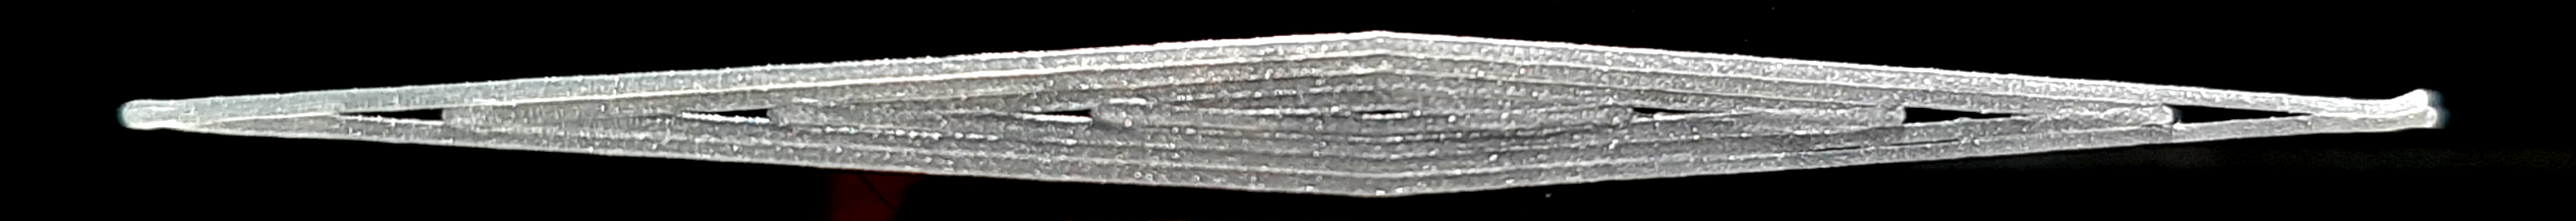
\includegraphics[width=\figwidth]{sources/applications/P3_print_wedge_naive_edited.png}
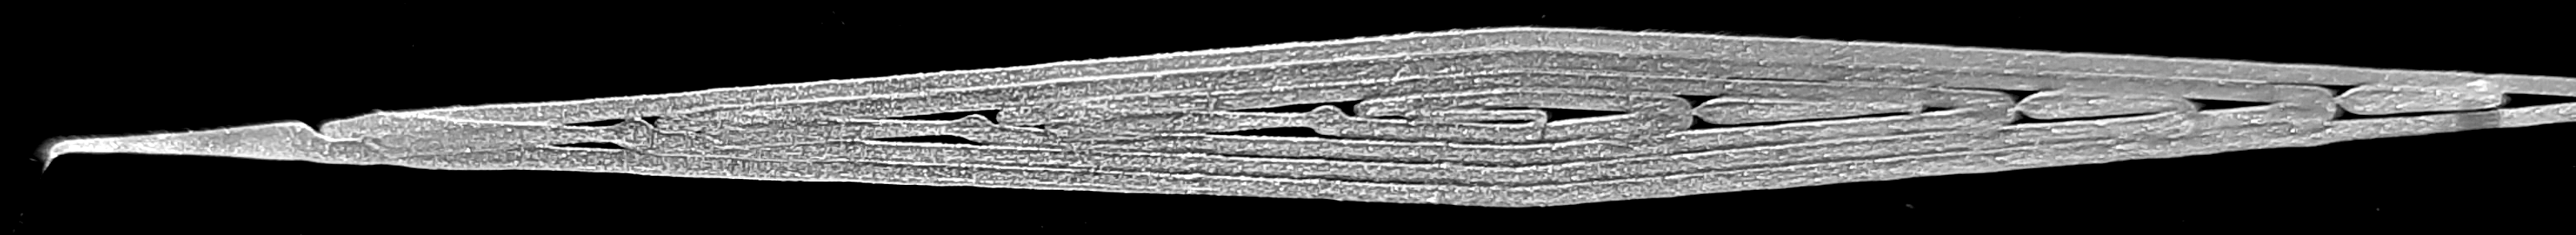
\includegraphics[width=\figwidth]{sources/applications/P3_print_wedge_center_edited.png}
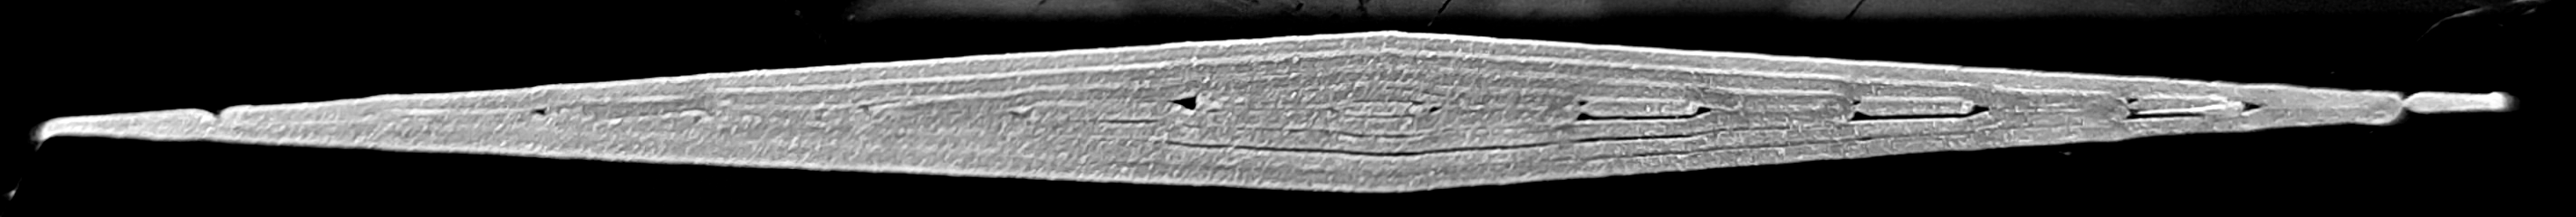
\includegraphics[width=\figwidth]{sources/applications/P3_print_wedge_inward_edited.png}
\caption{Wedge}\label{print_wedge}
\end{subfigure}
\caption{
A wedge shape printed using the naive strategy, center deivation strategy and the inward distributed strategy.
The wedge print can be read like a graph with model diameter on the X-axis and the resulting beads over the Y-axis.
The naive and center deviation strategy show problems around certain model diameters.
}
\label{wedge_print}
\end{figure}

\begin{figure}
\centering
\setlength{\figheight}{.38\columnwidth}
\setlength{\figwidth}{0.32\columnwidth}
\begin{subfigure}{\figwidth}\centering
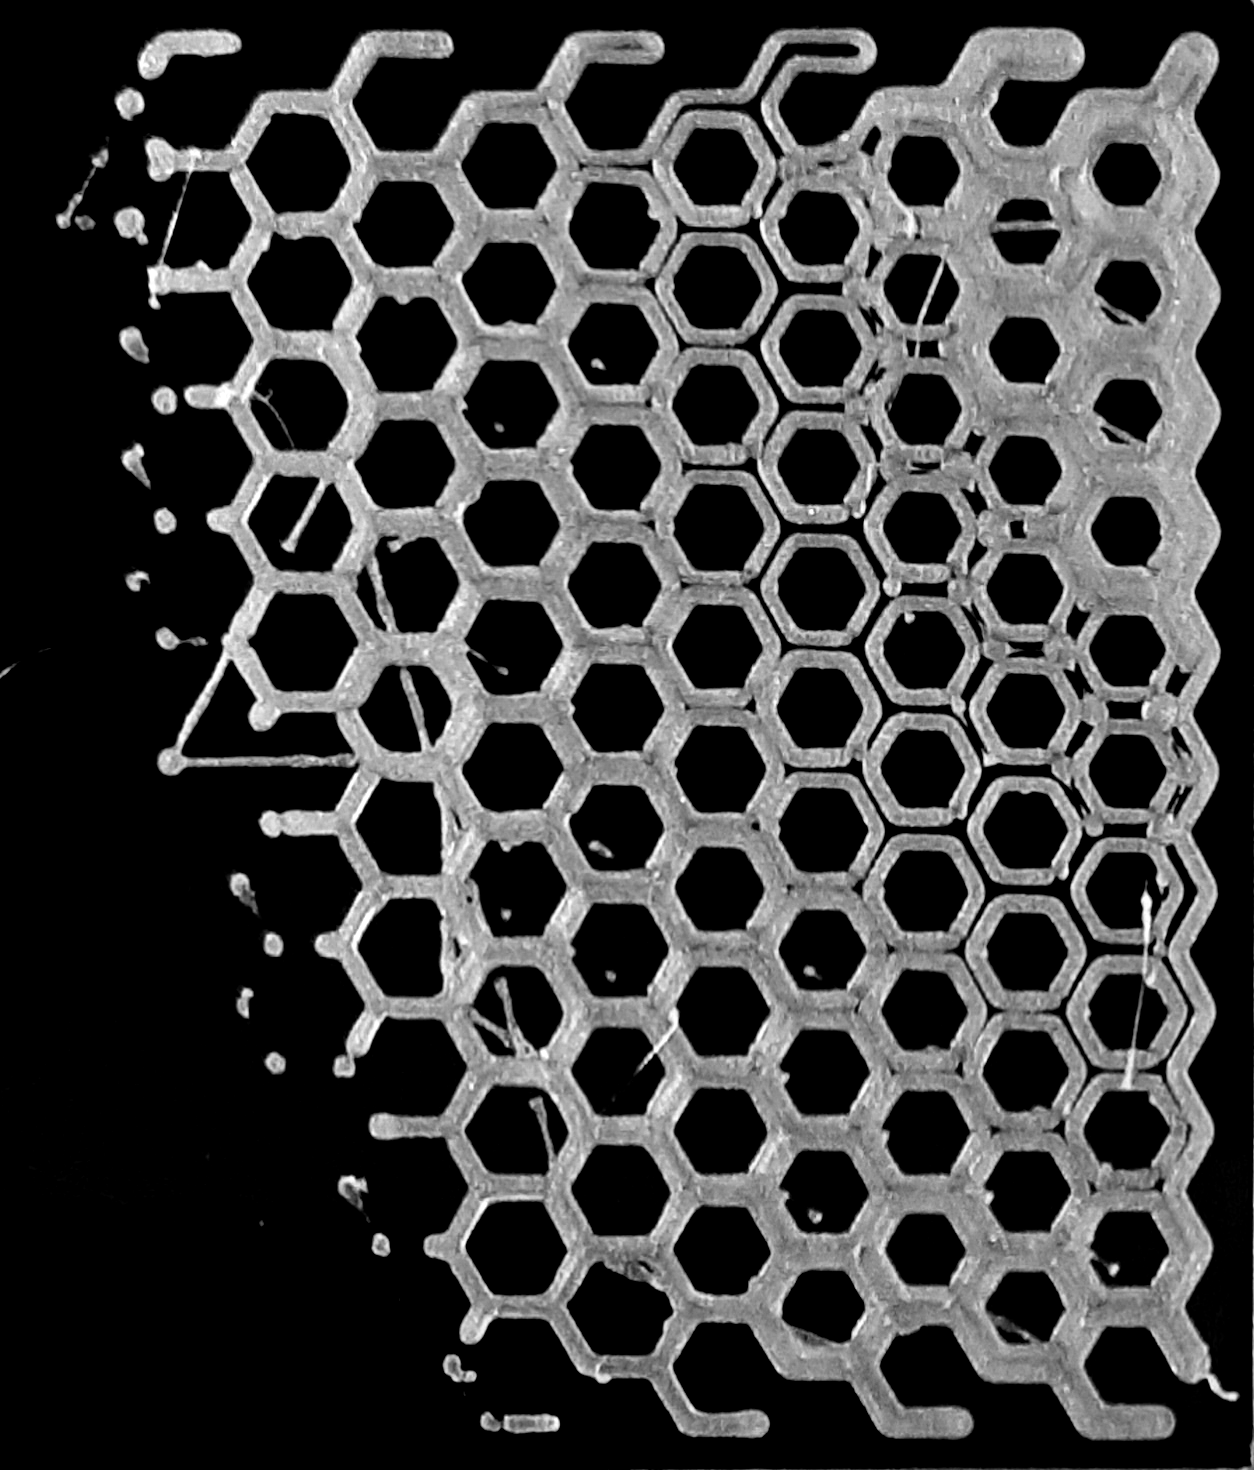
\includegraphics[height=\figheight]{sources/applications/P3_print_hex_naive_edited.png}

\includegraphics[width=\figwidth]{sources/applications/P3_print_UM_naive_edited.png}
\caption{Naive}\label{print_naive}
\end{subfigure}
\begin{subfigure}{\figwidth}\centering
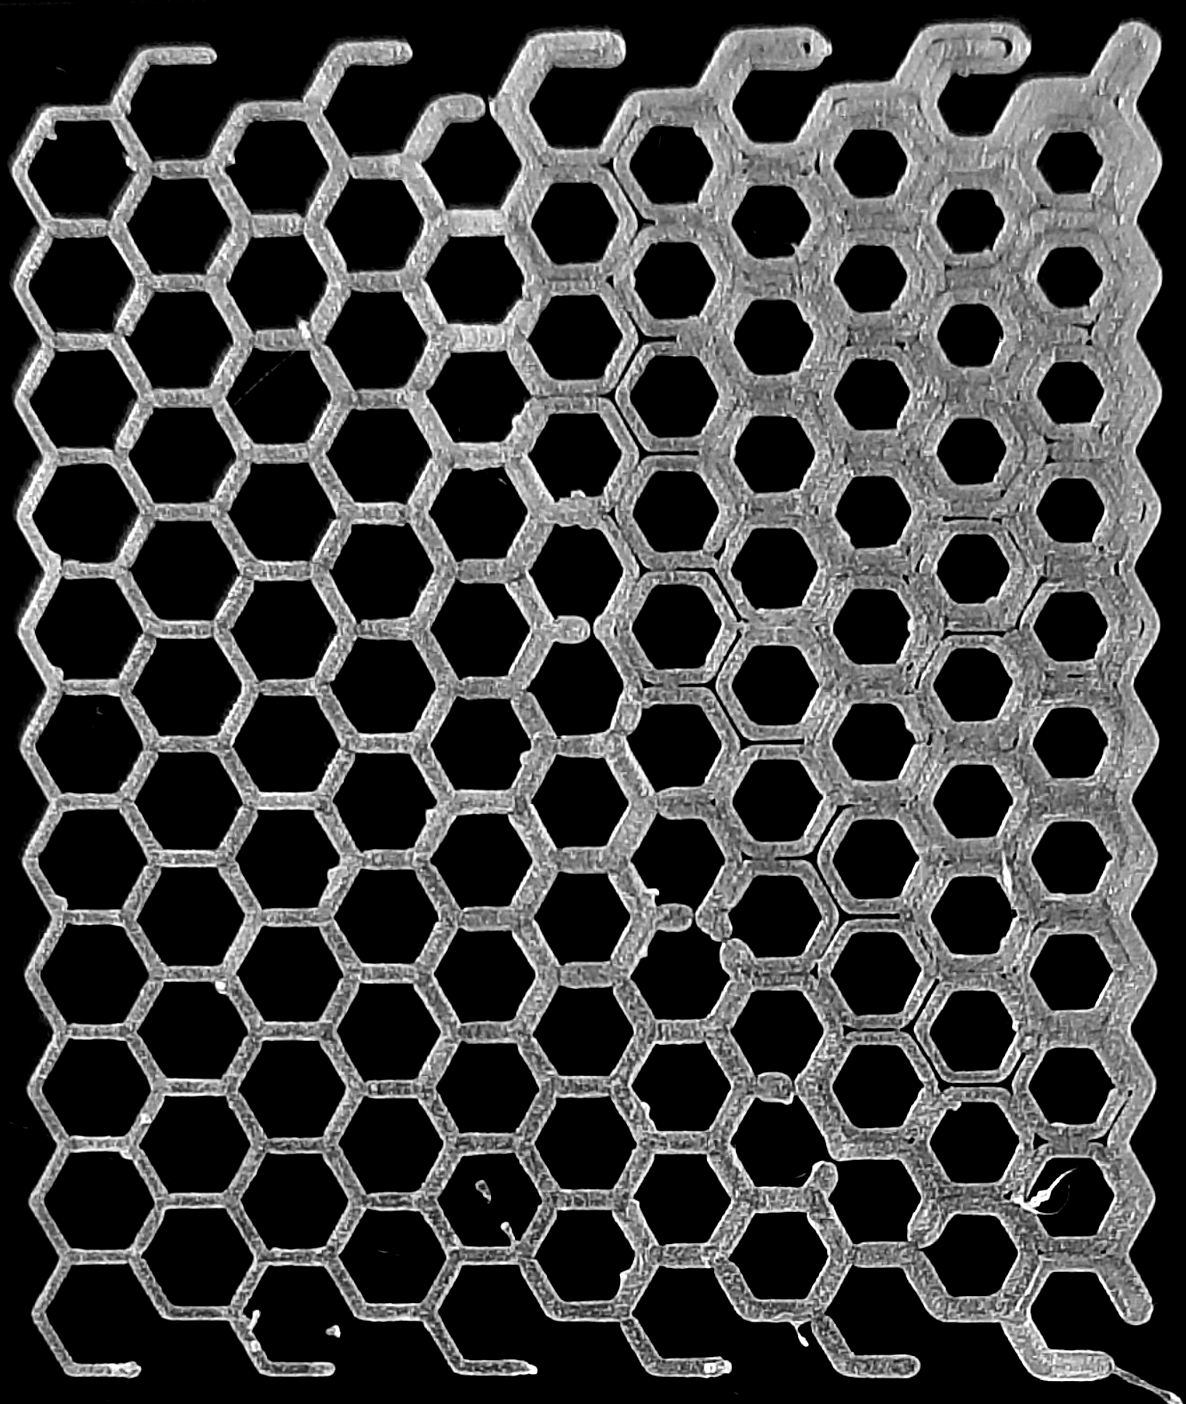
\includegraphics[height=\figheight]{sources/applications/P3_print_hex_center_edited.png}

\includegraphics[width=\figwidth]{sources/applications/P3_print_UM_center_edited.png}
\caption{Center deviation}\label{print_center}
\end{subfigure}
\begin{subfigure}{\figwidth}\centering
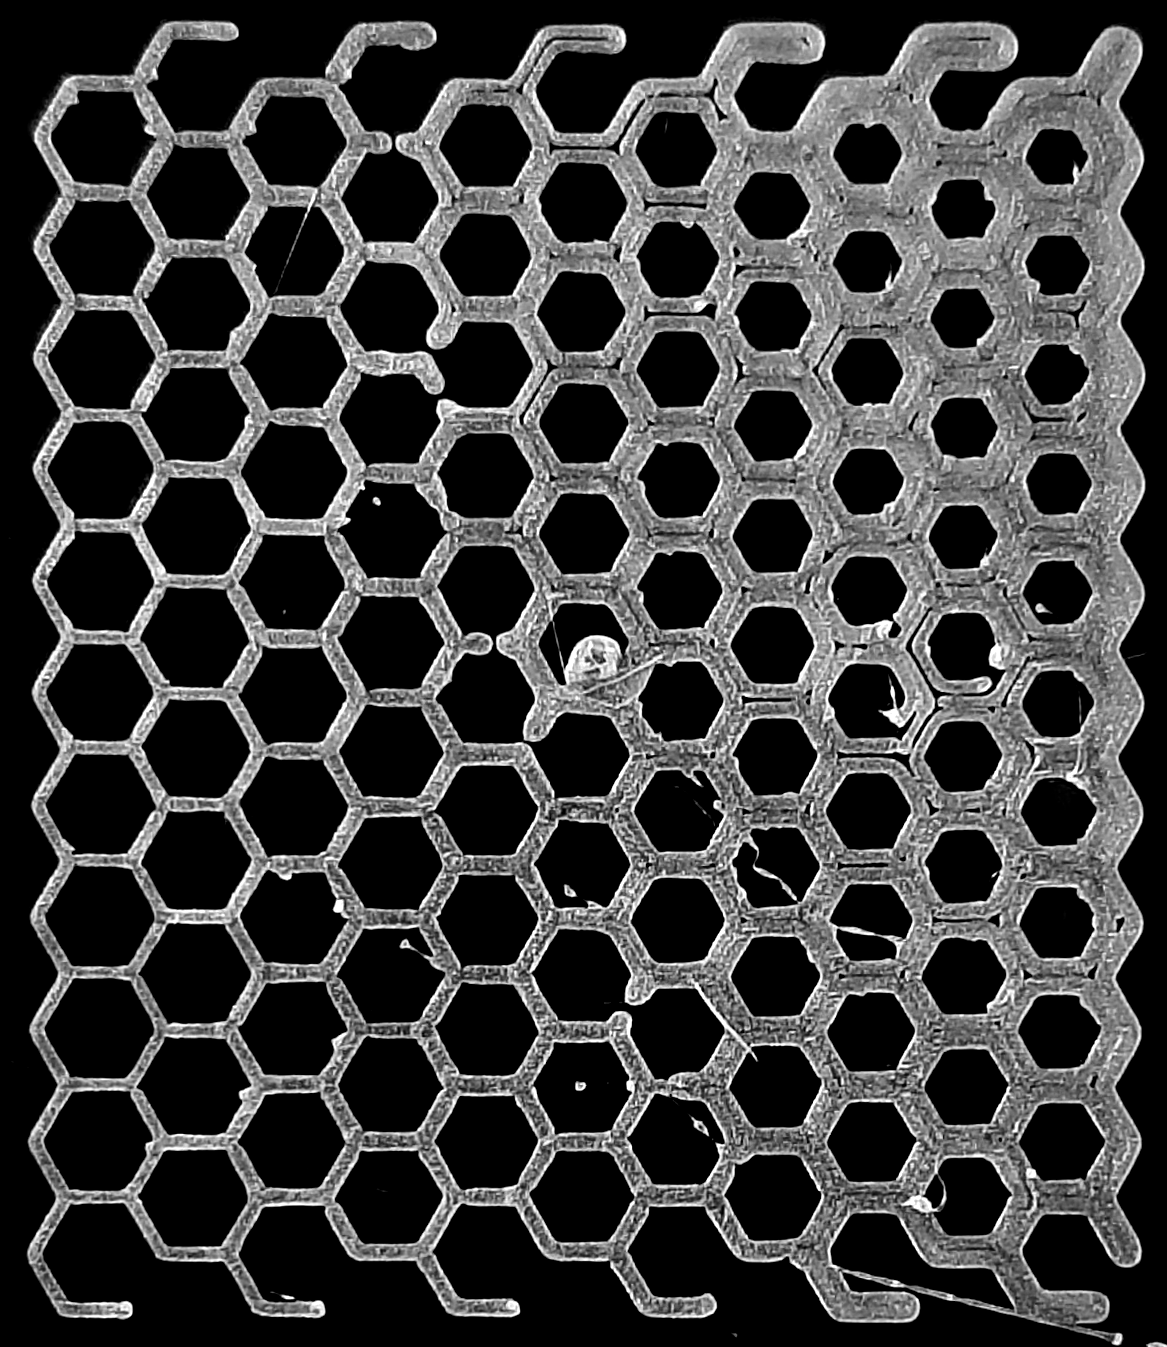
\includegraphics[height=\figheight]{sources/applications/P3_print_hex_inward_edited.png}

\includegraphics[width=\figwidth]{sources/applications/P3_print_UM_inward_edited.png}
\caption{Inward distributed}\label{print_inward}
\end{subfigure}
\caption{
Test shapes printed using the naive strategy, center deivation strategy and the inward distributed strategy.
The naive method produces distinct underfill areas.
The center deviation strategy shows some defects due to inaccurate control of extremal deposition widths.
The inward distributed strategy produces the least defects.
}
\label{prints}
\end{figure}


\iffalse
\todo{Maybe test the following qualities:}
\begin{itemize}
\item visual consistency of flat top skin surface
\item graphs of tensile tests on thin walled object
\end{itemize}
\fi










We therefore visualize include a semi-circle with a diameter equal to the starting width in the one end, and exclude it at the other end, because it will be included in the next extrusion segment.

